\documentclass[conference]{IEEEtran}
\IEEEoverridecommandlockouts
% The preceding line is only needed to identify funding in the first footnote. If that is unneeded, please comment it out.
\usepackage{cite}
\usepackage{amsmath,amssymb,amsfonts}
% \usepackage{algorithmic}
\usepackage{graphicx}
\usepackage{textcomp}
\usepackage{xcolor}

\columnsep 0.24in
\addtolength{\topmargin}{0.075in}
\addtolength{\textheight}{-0.1in}

\def\BibTeX{{\rm B\kern-.05em{\sc i\kern-.025em b}\kern-.08em
    T\kern-.1667em\lower.7ex\hbox{E}\kern-.125emX}}
\begin{document}

\title{Structural Assessment on Stateless Blockchain Improvements with
LRU-oriented Cache Replacement Policy}

% \author{\IEEEauthorblockN{1\textsuperscript{st} TSAI, TSUEN-JE}
% \IEEEauthorblockA{\textit{Department of Computer Science \& Information Engineering} \\
% \textit{National Taiwan University}\\
% Taipei, Taiwan \\
% r05922086@ntu.edu.tw}
% }

\maketitle

\begin{abstract}
Cryptocurrency based on blockchain is a peer to peer trading
system. In this decentralized system,
each node maintains a complete ledger which
records entire transaction history of all accounts.
Years after years, requirement to single node will
get higher and higher. Dealing with the issue, stateless
blockchain is a promising approach. To be more specific,
in this system, each transaction is attached with proof
of validity. With this approach, there is no need for a node
to access the data storage device to search past information
of the ledger. Instead, node only verifies the proof attached
to each transaction. Therefore, it will significantly
reduce the space of data storage for each node.
But it will cause additional network traffic and
verification time.

In this paper, we will discuss the following two points
on account-based blockchain.
First,
It is highly possible to infer the validity of
a transaction from another valid transaction appearing recently.
If we cache account information, we can eliminate some
proof in transactions and then reduce network traffic
and verification time.
Second,
There are so many cache replacement policies.
For LRU policies, we designed two composite data
structures which based on red-black tree and value-independent order tree.
And conduct some experiments to compare the costs of
cache hit with the penalty of cache miss.
Simulating today's Ethereum's block property,
when cache size can contain several tens of blocks' information,
the cache searching time is significantly lower than
the time to verify Merkle Patricia proofs.
\end{abstract}

\begin{IEEEkeywords}
blockchain, stateless blockchain, data structure
\end{IEEEkeywords}

\section{Introduction}
In 2008, Satoshi Nakamoto proposed the white paper
of bitcoin~\cite{b3}. It is a new type of cryptocurrency
system based on blockchain. In this system, each node
maintain a complete ledger in order to attain the
high degree of decentralization of entire system.
However, as the data size of ledger got bigger and bigger,
storage space of node increased yearly. Ten years later,
it costs hundreds of GB storage space for a node to run
some well-known cryptocurrency system, such as Bitcoin and
Ethereum~\cite{b4}. Thus, it gradually make the nodes maintained
by person overload. If we settle for second best by saving the
information needed for verifying new block, such as UTXO in
Bitcoin and world state in Ethereum, it still needs
several or tens of GB for disk storage place. With
this method, not only the storage space of disk is
requested but also  I/O speed. Furthermore, it is
too slow for traditional disk to access randomly.
The speed of verifying a block on Ethereum can't keep
up with the generation speed of blocks. It force the node
maintainer on Ethereum to buy expensive solid-state disk,
and it further cause the increase in operation cost of node.

To deal with the problem above, cryptocurrency communities
start trying several solutions, and stateless blockchain
is prospective one of them. It only need to store
block header for each node on stateless blockchain.
Nevertheless, each transaction must be attached with
proof of validity. This approach significantly reduces
the requirement of storage space. Furthermore, it is
no need to search the validity of transaction on disk;
namely, it drastically reduces the I/O time.

This paper proposes an improvement to stateless blockchain.
We let the node on stateless blockchain reach a consensus
to maintain a cache. If the payer of transaction appears
in recent transaction, it is highly possible to infer
the validity from cache. Hence, due to the omission of
proof of validity, it reduces the size of transaction and
the Internet traffic while broadcasting. However, how
to maintain cache effectively becomes a new problem.
When a new block append to the blockchain, there will be
a correspondent cache. Nevertheless, there will
also exist overlap on the blocks nearby.
Therefore, we design persisted data structure
for different cache strategies, such as the
nearest k blocks and LRU, and we conduct an
experiment to test their performance.

The remaining sections are arranged as follows.
section II illuminates the design of stateless blockchain,
including cache strategies and data structures
used by cache; Section III show the design and
results of experiments; Section IV narratives some related works,
and concluding remarks are found in section V.

\section{design}
In order to reduce occupied space of the disk, it is necessary for a stateless blockchain to attach a proof to each transaction. However, this move will increase Internet traffic. Furthermore, to reduce the time of accessing disk, it will cost computational power for CPU to verify the proof.
Compared to normal blockchain, stateless blockchain made some trade-offs. Regarding the purpose of shallow-state blockchain, the trade-offs are no longer all or nothing, which means that all transactions are attached with proofs or none of transactions are attached with proofs. It makes the degree of state storage adjustable.

\subsection{shallow-state blockchain}
In stateless blockchain, if payers and payees in some transactions are the same, the proofs in these transactions will be identical. It is obvious that the same proofs can be omitted in a block. Extended by this idea, if we cache the accounts’ information appearing in recent transactions, there is no need to verify the proof again when the accounts make transactions.

To go a step further, if nodes on the Internet follow the same set of rules to record cache, it will reach a consensus that node knows whether to attach the proof. While broadcasting the block, nodes can get rid of unnecessary proofs, and then reduce internet traffic.

\subsection{cache design}
We can make every node's cache the same by a simple design principle. Namely, each block has its own cache, and the content of cache depends on which chain the block is situated. Therefore, we turn a tree structure into a list, and it is definitely identical for the block on different nodes. If every node uses the same deterministic algorithm to compute the cache from this list, it can ensure that every node gets identical results of cache after verifying the same block.

\subsection{persistent cache}
We take an approach: every block retains its own cache. When a new block is about to append to the chain, it can directly use the cache of the previous block. Thus, there is no need to compute cache again. In other words, we adopt fully persistent data structure to store cache. Everytime the chain gets a new block, it creates a new version of cache.
In this method, we have to delete the cache of older blocks, such as the block 20 blocks far from the newest one, in order to limit the size of cache to a certain range. Otherwise, it will run out of memory, and it will violate our design principle.
Adopting this method leads to a new problem. If we duplicate the cache of the previous block, the space of cache will be proportional to the cache numbers that we didn’t delete. However, there is a high similarity of the cache in adjacent blocks. If we use appropriate data structure to have the cache shared by adjacent blocks, it will effectively increase space usage.

\subsection{LRU}
LRU is an acronym for “least recently used”.
In this strategy, the size of cache is fixed.
If a cache is full, it will discard a piece of data before inserting new data.
In LRU strategy, the least recently used data will be discarded.
The reasons why LRU has higher hit rate than FIFO are revealed by the history data of Ethereum.
First, after an account spends money,
it is highly possible that it will spend money again.
Second, after an account receives money,
it is highly possible that it will spend money right away.
Because LRU updates the using time of data,
it is able to keep caching the data appearing frequently.
However, FIFO only looks at the coming time of data.
Even if some data appear frequently,
they will be discarded sooner or later.

From an abstract view, LRU is a data structure that supports two kinds of interface.
\begin{itemize}
\item get(key)
\item put(key, value)
\end{itemize}
When executing get(key), LRU will determine whether the key exists. If the key exists, it will return the value and update its using time.
When executing put(key, value), LRU will determine whether the space of LRU is full. If the space of LRU isn’t full, the key-value pair will be inserted to the space directly.  If the space of LRU is full, LRU will find out the least recently used one in the cache and abandon it, and then insert the new key-value pair to it. The using time of the new key-value pair should be the latest.
Corresponding to the situation of stateless blockchain, every time when a new block appends to the chain, we have to compute the cache of the new block. In this time, a series of read and modify execution of accounts will turn into get and put. Key will be the address of account, and value will be the state of account. Finally, the underlying data structure of LRU will take the correspondent action.

\subsection{persistent LRU algorithm}
Before discussing persistent LRU algorithms, we first observe how to efficiently implement LRU cache on software. Judging from several popular LRU libraries on github, interior data structures are all combinations of hash table and doubly linked list.
While executing get, it will get the data by the pointer pointing to the node of list. Then, the node will move to the head of the list. While executing put, if cache hits, the value of node will be updated, and the node will move to the head of the list. If cache is not full, the cache value will be added to the head and the pointer will be put in the hash table. Instead, if the cache is full, pull out the tail node of the doubly linked list, and delete the old key in the hash table. Then, add cache value to the head and put the pointer in the hash table.
We observed that there are two kinds of information that need to be recorded by LRU.
\begin{enumerate}
  \item find the value from key (key-value pair)
  \item the order information of all keys
\end{enumerate}
In the implementation of combinations of hash table and doubly linked list, hash table is responsible for (1), and doubly linked list is responsible for (2). We observed that a doubly linked list records the order relationship naturally, and it doesn't even need to record the definite using time.
There is one simple idea that we directly combine persistent-versioned alternatives of a hash table and a doubly linked list, and then we get a persistent LRU. Although there are mature alternatives~\cite{b5}~\cite{b6} for hash tables, it is hard to find such a thing for doubly linked lists.
Thus, we need to use other persistent and efficient data structures to replace doubly linked lists. The things that an abstract doubly linked list can do are as follows.
\begin{itemize}
\item Update the using time of node to latest
\item Delete the least recently used node
\item Insert new node and update the using time of the node to latest
\end{itemize}
Following we will discuss how to use red-black tree~\cite{b7} to complete the above tasks and introduce our design of value-independent order tree, which is more efficient than red-black tree.

\subsection{hash table + red-black tree}
We tried to use red-black to record the order information.
First, set a unique timestamp for every account.
This timestamp is easy to access. For instance,
it could be $block\_height * max\_tx\_in\_one\_block+ tx\_number$.

Afterwards, build a red-black tree whose key is timestamp and value is account’s information. About hash table, the account's address is set as key and the correspondent timestamp is set as value.
While executing get, it first gets the timestamp from the account's address in the hash table, and then gets the account’s information from the timestamp in the red-black tree. For example, in Fig 1, we first get the account’s timestamp, 243, from the hash table, and search 243 in red-black tree.
After searching, it needs to update the using time. The specific operations are that modify the timestamp corresponding to the address in the hash table and remove the original node in red-black tree. Then, set the new timestamp as key. The put operation is similar to get operation. However, it needs to modify the account's information. 
Fig 2 shows the sharing structure of the persistent red-black tree. In this figure, the cache size is 8. In state 1, there are only 7 data. After that, state 2 insert 14 in it, and there are 8 data. State 3 insert 15 to state 2, and the cache is full. Therefore, it has to delete the data of minimum timestamp; that is, the red 7 at lower left corner will be deleted.

\begin{figure}
  \centering
  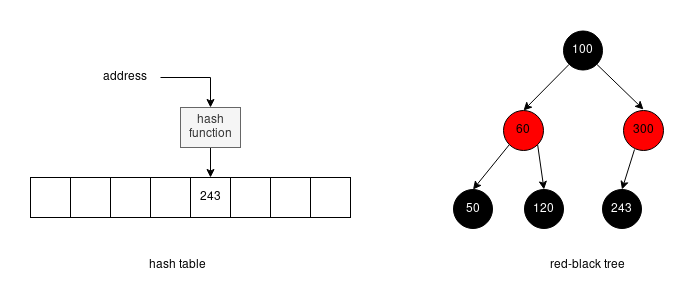
\includegraphics[width=0.4\textwidth]{../images/ht-rb-tree}
  \caption{hash table + red-black tree}
\end{figure}

\begin{figure}
  \centering
  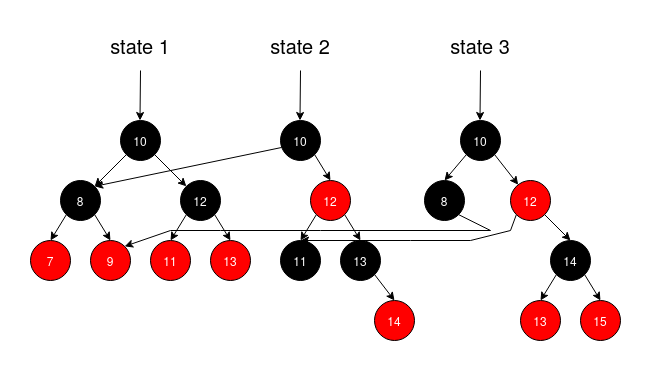
\includegraphics[width=0.4\textwidth]{../images/immutable-rb-tree}
  \caption{immutable red-black tree}
\end{figure}

\subsection{hash table + value-independent order tree}
Doubly linked list records order relations by the pointer relations of nodes. Red-black tree has to additionally record the timestamp. Moreover, the account’s information that we can search with the hash table in one time now needs two steps with red-black tree; namely, we find the timestamp from the address, and then find the account's information from the timestamp.
The reason why doubly linked lists cannot turn into persistent data structure through path copying is that two adjacent nodes always point to each other. Once modifying the node by path copying, it has to copy the whole list. Therefore, we want to find another way to connect the nodes.

Image to weave a net behind the nodes, and then stick them together.
The basic form of the net structure is a full binary tree. We name the structure using a full binary tree to store order data as value-independent order tree. We will introduce the operations of value-independent order tree as follows.

If cache size is n, the height of the value-independent order tree will be set as 1 + log n. That is to say, the number of leaves is at least two times the cache size. Fig. 3 shows that there is an value-independent order tree with size 4, and it has 8 leaf nodes.

Applying to LRU cache, the value stored by the hash table is a pointer pointing to the leaf node of the value-independent order tree. It only needs one time to get the data by searching the hash table. 
value-independent order tree stores the entire data in leaf nodes, and each data is arranged in the order of time. In this paper, the newer the data, the more the right side of the leaf position. We will explain and draw in this way.

Some leaf nodes in the value-independent order tree have stored data, while some of them haven’t. We call the leaf with data as “used leaf”, and the leaf without data as “unused leaf”.
While executing get, change the used leaf into an unused leaf if it has been searched, and then write the data of the original leaf to the unused leaf on the right side of the rightmost used leaf. While executing put, first find the leftmost used leaf and change it into unused, and then write the data of the original leaf to the unused leaf on the right side of the rightmost used leaf. No matter get or put, it always occupies a leaf on the right. If the used leaf is on the rightmost of the tree, it has to execute full copy. Therefore, make all the used leaves tightly packed together to the left side of the new value-independent order tree in the original order.

Fig. 4 shows a series of execution of value-independent order tree. In this figure, full copy happens at the time when state 6 turns into state 7. The light blue nodes in the figure mean that they are unused. Notice that we painted all unused leaves of subtree light blue.
In implementation, there is no need to allocate memory space to light blue nodes. The pointer pointing to light blue subtree is a null pointer.

\begin{figure}
  \centering
  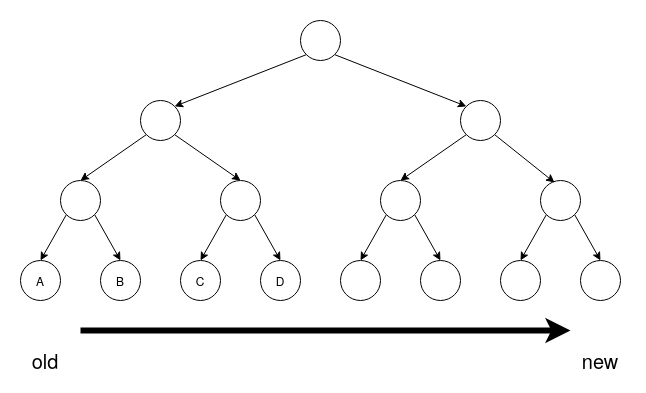
\includegraphics[width=0.4\textwidth]{../images/order-tree}
  \caption{value-independent order tree with size 4}
\end{figure}

\begin{figure}
  \centering
  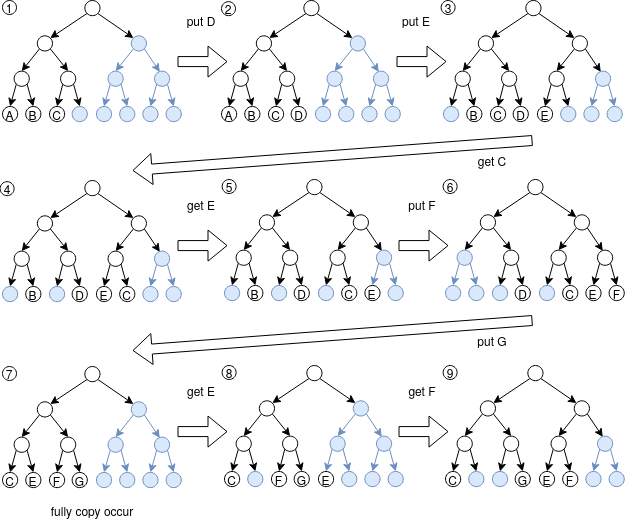
\includegraphics[width=0.4\textwidth]{../images/order-trees}
  \caption{value-independent order tree multiple operation}
\end{figure}

\subsubsection{complexity analysis}
In the following analysis, the size of the value-independent order tree is $n$.
If full copy doesn’t happen, execution of get and put go through root to leaf two times.
The height of the value-independent order tree is $O(\log n)$, and the time and space complexity are both $O(\log n)$.  

If full copy happens, it has to go through the value-independent order tree,
and has all used leaves congregate to form a new tree.
Notice that the total number of nodes of a full binary tree is two times the quantity of leaves minus one,
and the total number won’t exceed $8*n$.
Therefore, the time and space complexity are both $O(n)$.

It may be a little high for the $O(n)$ complexity.
However, everytime when operating get or put only
make the used leaf move one grid to the right.
It costs  at least n operations for the used leaf
to go to the rightmost of the tree. Thus, if the
cost of full copy is amortized to every operation,
the time and space complexity are both $O(1)$,
and time and space complexity of get and put are still $O(\log n)$.

\section{experiment}
In this section, we evaluated the performances of 
persistent LRU implemented in different data 
structures under different workload.

\subsection{Experiment Environment}
All experiments were all conducted on the workstation below:

\begin{itemize}
\item CPU: AMD Ryzen 7 2700X (8 cores 16 threads, 3.6 GHz, 32K L1d cache, 64k L1i cache, 512K L2 cache, 8M L3 cache)
\item memory: DDR4 64 GB
\item OS: Linux manjaro 4.19.36-1-MANJARO x86\_64
\item compiler: GCC 9.1.0
\end{itemize}

\subsection{Data Structures}

We use C++ 17 implemented three data structures:

\begin{itemize}
\item hash table + doubly-linked list, it will copy itself when creating a new version
\item persistent hash table + persistent red-black tree
\item persistent hash table + persistent value-independent order tree
\end{itemize}

Because what we want to simulate is blockchain,
all workload use block as unit.
There are many get/put instructions in a block.
To optimize this kind of workload,
the persistent data structures described above all
support transience. That means data structure doesn't 
generate a new version for every get/put instruction,
but generate an temporary ephemeral data structures and
make it immutable one after operating batch of instructions.
While eliminating lots of intermediate states,
this optimization can significantly improve performance.

We claim that, in our implementation:
Hash table is unordered\_map in C++ standard library.
For persistent hash table, we use famous C++
persistent data structures library immer.
Doubly-linked list, persistent red-black tree,
persistent value-independent order tree are all implemented by ourselves.

From now on, we will refer to these three composite data structures
as doubly linked list, red-black tree, and value-independent order tree.

\subsection{performance}

\subsubsection{workload}
We use a simple model to simulate block generation,
there are n nodes in the network,
Each node will mine for the highest block
(that is, the top of the longest chain it recognizes).
Initially, The highest block of each node
is genesis block. Afterwards, there were several rounds,
In each round, each node has a certain probability
to dig out new blocks. If it is not dug,
It will go to the successor block of the
highest block dug by other nodes,
if the highest block does not have any successor block,
node will randomly go to other longest chains.
If no node has dug out any block,
the same process will be repeated.

In all workloads, it is assumed that there
are 10 nodes in the network, and the probability
of each node to dig out new block in one round is one-tenth.
The block generating process will stop after mining 1000 blocks.
Under this setting, there will be about
1.5 blocks at the same height.

From etherscan, we can
know that Ethereum's gas limit is about ten million, and
it will cost 21000 gas fee per transaction.
After simple division, a block can contain about 500 transactions.
Therefore, the number of get/put instructions
for one block of our workload is set to 500.

In addition, There is another argument, get/put rate.
For normal ethereum transaction,
payment always results in state changing,
but it's not true when smart contract is involved.
Therefore, it is possible get/put instructions both appear.
If there is no additional explanation below,
the put instruction will account for 50 \% (get instruction also accounts for 50 \%).

Before starting any task, we will first fill
the entire cache, if not, when the cache size is set too large,
workload takes a long time to fill it up,
and the state when the cache is not full is not our concern,
as the blockchain is usually composed of millions of blocks,
For most of the time, the cache is full.

\subsubsection{Adjust Cache Size}

The first experiment fix hit rate to 100\%,
and adjust the size of cache (the number of key-value pairs).

\begin{figure}
  \centering
  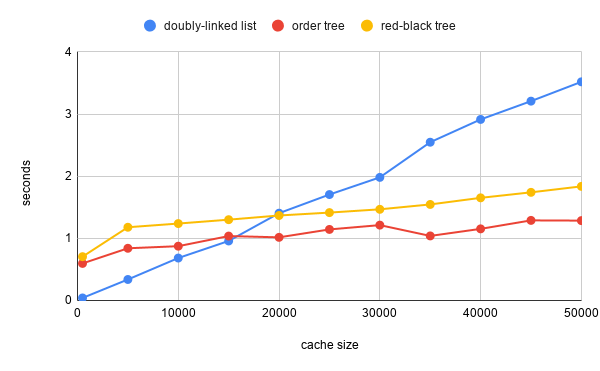
\includegraphics[width=0.4\textwidth]{adjust_cache_size.png}
  \caption{adjust cache size}
\end{figure}

In Fig. 5, we can see that time cost by doubly-linked list
is proportional to the cache size. It's because that
the main cost of doubly-linked list is on replication.
How big is the cache, how much is the amount to be copied each time the block is updated

The growth curve of the red-black tree and the sequence
tree is rather gentle ($O(\log n)$).
Noting that the line graph of the value-independent order tree,
compared to the smooth growth of the red-black tree,
is somewhat oscillating,
Because the number of leaves of the
value-independent order tree is $1 + \lceil \log_2 n \rceil$,
its number of leaves is more discrete,
When the cache size reaches the power of $2^k$,
the number of leaves doubles, which will affect
the performance and cause oscillating.

\subsubsection{Adjust hit rate}

In this experiment, we fix cache size to 30000, and adjust hit rate.

\begin{figure}
  \centering
  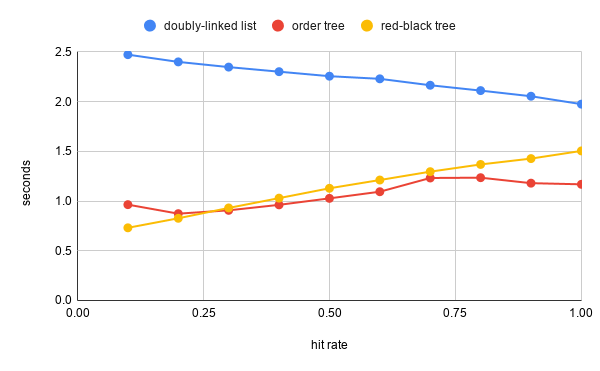
\includegraphics[width=0.4\textwidth]{adjust_hit_rate.png}
  \caption{adjust hit rate}
\end{figure}

In Fig 6, we can see that the hit rate has no effect
on the doubly linked list, because its main consumption
comes from replication, the only thing to do
after the cache hit is to move a few pointer,
it doesn't take much time.
The time consumption of red-black trees and order
trees will increase with the increase of hit rate.
Because their main time-consuming comes from path copying,
the more cache hits, the more branches need
to be copied and created.

\begin{figure}
  \centering
  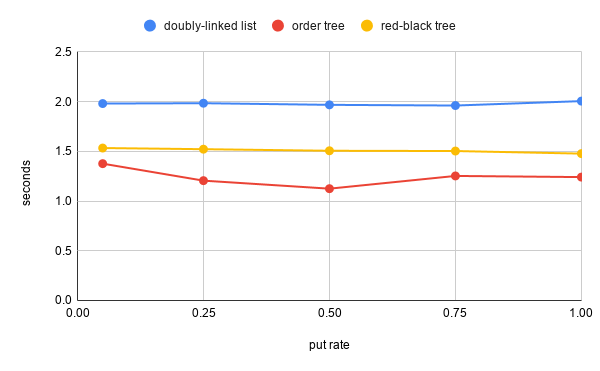
\includegraphics[width=0.4\textwidth]{adjust_put_rate.png}
  \caption{adjust put rate}
\end{figure}

Set the cache size to 30000, the hit rate to 1.0,
and adjust the proportion of put in the get/put instructions.
It can be seen from Figure 7 that the performance
is basically not affected.

\subsection{Miss Penalty}

When verifying a transaction whose related account information
is not in the cache of the node (cache miss),
This transaction must be accompanied by a proof
for verification. Therefore, There are two penalties when cache miss:
(1) It cost network I/O to receive the proof, which is directly related
to the size of the proofs.
(2) The CPU execution time consumed by the proof verification.

From Fig 7 we can know that, when cache size is 30000,
put rate is 100\%, hit rate is 1.0, value-independent order tree implementation
can process 1000 blocks in 1.241 seconds, that means 
the average time to process a block is 1.241 milliseconds.
This number will be smaller when the cache size is smaller.

We chose Merkle Patricia tree verification cost to compare
with the value-independent order tree implementation,
We choose trie-db module,
which is a part of one of the two major
Ethereum implementations,
Parity Ethereum, to conduct experiment.

There are two factors that influence
Merkle Patricia proof's verification performance:
(1) If the number of leaves is $s$,
the size of the proof is about $O(\log s)$.
The time complexity of verifying a proof is also $O(\log s)$.
(2) The number of proof in one batch.
A Merkle proof is a branch of the Merkle tree.
When a node is shared by multiple branches,
there is no need to repeat calculations.
So the time to verify $k$ proofs at a time will be
shorter than $k$ times the time to verify a proof.

By the information of etherchain.org,
the number of Ethereum accounts today has exceeded 80 million,
So we first randomly insert 80 million pieces
of data into the Merkle Patricia
tree (that is, the number of leaves is 80 million),
And based on the assumption of 500 transactions in
one block, we batch verify 500 proofs at a time,
The measured time is 5.536 milliseconds, which is
obviously more time-consuming than direct access to cache.

In the aspect of I/O overhead, the proof size of a
block is about 900 KB, and 1000 blocks is almost 900 MB.
If we use the common home network today,
the time required to download these additional
proof is more time-consuming than verifying the proofs.

\subsection{Experiment Conclusion}

The Experiments verify that value-independent order tree and red-black tree
have lower time complexity. When the cache size increases
to a certain extent, they significantly beat ever-copy
doubly linked list in performance. Compared with
red-black tree, value-independent order tree does not need to maintain
the color of the node, and to execute various rotation rules,
There is a little advantage in execution speed.

At the same time, we also experimented and measured
the proof size and verification speed of the Merkle
Patricia tree. Understand that under normal circumstances,
reading the cache directly is faster than downloading
and verifying the proof. Based on these data,
it can be deduced that if Merkle Patricia tree
is used as vector commitment, if the shallow state
blockchain adopts an appropriate cache size, it
can bring speed improvement under the LRU strategy.

\section{Related Work}
\subsection{Utreexo}
Utreexo~\cite{b1} applying the Merkle forest to  design a new accumulator.
Based on this accumulator, the Utreexo node does not need to actually store all of the UTXO and is still able to verify the blocks.

However, the bitcoin network has been around for years, and it's not realistic to drastically modify the protocol so that all nodes become stateless.
Utreexo proposes that a bridge node could be used as an intermediary between the bitcoin full node and the Utreexo node.
When the block broadcasts from the Utreexo node to the full node, the proof is stripped away, on the other hand, the proof is placed.

The paper also mentions that, analyzing the historical record of bitcoin
About 40\% of UTXO will be consumed in 20 blocks.
Nearly 80\% of UTXO will be consumed in 1000 blocks.
So by using a small amount of memory space to cache the most recent UTXO, you can skip transmitting many proofs.

The difference from this study is that this study considers account-based cryptocurrencies, rather than UTXO-based ones.
At the same time, this study additionally considers the situation when bifurcation occurs.

\subsection{Making Data Structure Persistent}

The paper~\cite{b2} proposes a variety of algorithms that enable any node-based data structure to be partial/fully persistent.
According to the node-splitting algorithm of that paper, it is even possible to complete the insertion and modification of a doubly linked list within the $O(1)$ time complexity.

However, the paper does not propose a way to remove older versions of the persistent data structure.
This makes it difficult to apply these algorithms to the caching of shallow state blockchains.
Because the inability to delete past versions will result in the space needed for caching never being released.

\section{Conclusion}
This paper describes the design of shallow state blockchain and discusses the advantages and disadvantages of multiple cache strategies.
Especially for the LRU cache strategy, 
we first try the combination of persistent hash table and persistent red-black trees,
Further proposed a novel data structure, value-independent order tree, let it be combined with persistent hash,
Get a more efficient implementation of persistent LRU.

\begin{thebibliography}{00}
\bibitem{b1} Dryja, Thaddeus. Utreexo: A dynamic hash-based accumulator optimized for the Bitcoin UTXO set. Vol. 2019. IACR Cryptology ePrint Archive, 2019.
\bibitem{b2} Driscoll, James R., et al. "Making data structures persistent." Proceedings of the eighteenth annual ACM symposium on Theory of computing. 1986.
\bibitem{b3} Nakamoto, Satoshi. Bitcoin: A peer-to-peer electronic cash system. Manubot, 2019.
\bibitem{b4} Wood, Gavin. "Ethereum: A secure decentralised generalised transaction ledger." Ethereum project yellow paper 151.2014 (2014): 1-32.
\bibitem{b5} BAGWELL, Phil. Ideal hash trees. 2001.
\bibitem{b6} Stucki, Nicolas, et al. "RRB vector: a practical general purpose immutable sequence." Proceedings of the 20th ACM SIGPLAN International Conference on Functional Programming. 2015.
\bibitem{b7} Guibas, Leo J., and Robert Sedgewick. "A dichromatic framework for balanced trees." 19th Annual Symposium on Foundations of Computer Science (sfcs 1978). IEEE, 1978.
\end{thebibliography}
\vspace{12pt}

\end{document}
